\documentclass[UTF8]{ctexart}

\usepackage{fancyhdr}
\usepackage{titlesec}
\usepackage{geometry}
\usepackage{ctexbook}
\geometry{a4paper,left=2cm,right=2cm,bottom=2.5cm,top=2.5cm}
\usepackage{graphicx}
\usepackage{epstopdf}
\usepackage{listings}
\usepackage{indentfirst}
\usepackage{multirow}
\graphicspath{ {figure/} } 

\pagestyle{fancy}
\lhead{} 
\chead{\bfseries 光信息科学与技术实验} 
\rhead{} 
\lfoot{} 
\cfoot{\thepage}
\rfoot{} 
\renewcommand{\headrulewidth}{0.4pt} 
\renewcommand{\footrulewidth}{0.4pt}

\newcommand{\major}{计算机应用技术,精密仪器及机械}
\newcommand{\name}{杜沈达,王晨}
\newcommand{\stuid}{SA18168163,SA18168095}
\newcommand{\newdate}{\today}
\newcommand{\loc}{物理楼}
\newcommand{\course}{光信息科学与技术实验}
\newcommand{\grades}{}
\newcommand{\newtitle}{单光子计数实验}

\makeatletter
\newcommand{\figcaption}{\def\@captype{figure}\caption}
\newcommand{\tabcaption}{\def\@captype{table}\caption}
\makeatother
\setlength{\parindent}{2.45em}

\begin{document} 
	\thispagestyle{empty}
	\begin{figure}[h]
		\begin{minipage}{0.6\linewidth}
			\includegraphics[width=\linewidth]{head.jpg}
		\end{minipage}
		\hfill
		\begin{minipage}{.4\linewidth}
			\raggedleft
			\begin{tabular*}{.8\linewidth}{ll}
				专业: & \underline\major   \\
				姓名: & \underline\name    \\
				学号: & \underline\stuid   \\
				日期: & \underline\newdate \\
				地点: & \underline\loc
			\end{tabular*}
		\end{minipage}
	\end{figure}
	
	\begin{table}[!htbp]
		\centering
		\begin{tabular*}{\linewidth}{llllll}
			课程名称: & \underline\course   & 
			实验名称: & \underline\newtitle & 
			成绩:     & \underline\grades \\
		\end{tabular*}
	\end{table}
	
	\titleformat*{\section}{\large\bfseries}
	\titleformat*{\subsection}{\normalsize\bfseries}
	\titleformat*{\subsubsection}{\normalsize}
	
	基于光的量子性,单光子测量技术是到目前为止最灵敏的弱光测量技术。一般来说,它比锁相放大技术的信噪提高三个数量级左右。因此几乎所有与极弱光信号相关的测量实验中都采用单光子计数实验。近十年内量子计数得到了迅速的发展,关于光子操控和检测技术是其核心的实验手段。在它的推动下,但光子操控和检测手段也正在迅速发展之中。现在常用单光子测量技术的科研领域包括:
\CTEXnumber{\test}{100002005}
	\begin{enumerate}
		\item 荧光、时间分辨光谱与拉曼光谱技术;
		\item 激光雷达系统;
		\item 激光 Doppler测速系统;
		\item 光子相关和光场分布测量;
		\item 量子信息学;
		\item 其他弱光检测领域。
	\end{enumerate}
\section{实验目的}
本实验是为高年级本科生和研究生开设的基本实验原理和技术课程,通过本实验,希望同学们得到这样一些实际的训练。
\begin{enumerate}
	\item 了解光量子性的物理实质;
	\item 掌握光电倍增管工作原理及特性,特别是单光子测量脉冲工作特性;
	\item 掌握单光子计数技术的基本方法、技巧以及适用范围;
	\item 了解暗计数和几种不同来源以及对应的处理方法。
\end{enumerate}
\section{实验原理}
通常信号的测量放大都不可避免这样三种噪声(热噪声、1/$f$、和量子噪声)的限制,导致微弱信号的信噪比有限,从而无法测量某些极弱的(光)信号。唯象地理解,弱光束可以被看成是一组不连续(离放)的光子流,该光子流的流量变化就代表着该光束强度的变化。如果我们有办法能够统计出光束截面上每秒种通过的光子数,我们就能够知道光束强度的变化,而且不会受到上述前两种噪声的限制,测量灵敏度就会更高。光子计数计数正是实现这种思路的一种方法。

单个光子的能量很低,要想探测到单个光子,必须使用极灵敏的光探测器,并在探测器内实现对单个光子信号的放大,才能让后续电路检测的光子脉冲。通常这个放大倍数不小于${EMBED Equation.DSMT4}$倍。为了达到上述目标,可见到1微米波段的光灵敏器件通常采用光电倍增管,而在通讯波段则使用过偏置雪三极管,这里以光电倍增管为例当一个光子入射到光阴极上时,它有一定的概率(决定于光阴极的量子效率)靠外光电效应发射出一个光电子,光电倍增管通过它的特殊结构,使光电子以几何级数倍增,放大了>10倍的电子束在阳极回路中形成一个光电子脉冲。后续电路只要检测并记录这个光电子脉冲就可以实现计数光子的目的。

可能干扰此过程的会有这样一些原因:

尽管放大了很多,单光子光电脉冲信号仍然很弱,因此,较大的外界干扰和噪声都会使得我们无法区分光电子脉冲和干扰或噪声脉冲,因此要尽可能减少外界干扰和电路本身的噪声。

暗计数,暗计数就是在没有任何光子落在光阴极上,但光电倍增管仍然输出的“光”电脉神。它主要有这样两个来源。

其一:光电倍増管的阴极和各打拿极都会因为热发射而有电子逃逸出来,在光电倍增管的加速电压驱使下,同样会在阳极形成电脉冲,这个脉冲是在没有光的情况下产生的,所以称之为暗计数。事实上,除了阴极的热电子发射以外,其他各打拿极热发射形成的暗脉冲都要比光电子脉冲低,因为从阴极后的第一打拿极开始,各极的热激发电子到达阳极时的放大倍数成几何级数依次递减。因此,为抑制这种暗计数的干扰,通常在后续电路中增加值甑别器,目的之一是只让脉冲高度大于某个阈值的脉冲通过,另一目标是将光电倍增管的输出脉冲成形,能精确并触发后续电路计数,而小于该阈值的脉冲则作为暗计数屏蔽掉,但是,不论是什么情况下产生于阴极单个光电子形成的脉冲与实际的光子脉冲都无法区分,因此也就不可能用甑别的办法消除计数。

其二:来自于空间的各种高能辐射粒子以及光电倍增管内部剩余气体离子。高能粒子通常不会被简单的密闭挡光金属盒子所遮蔽,可以直接作用到光电倍增管的阴极,触发“光”电子脉冲;而残余气体的离子带正电,而通常使用的光电倍增管阴极为负电位,由于这种“粒子”的能量一般比光子能量大,可以在阴极上一次激发两个以上的“光”电子,由此形成的“光”电子脉冲比前一种暗脉沖要高,通常比真正的光电子脉冲还要高。所以要求严格的光子计数系统的甑别器有两个阀值,其中上阀值就是用来屏蔽那些高于某电平的脉冲,只让高度介于两个电平中间的光电子脉冲通过。好在通常的空间辐射脉冲数量较少,优秀的光电倍增管的这种离子也很少,一般要求不高的系统,不加上甑别阀值所引入的误差也是可以忍受的。

如上图所示,原则上,光电倍增管输出的脉冲幅度低于A电位的是各打拿极的发射;脉冲幅度在A和B之间的是光子信号脉冲和阴极热发射,而高于B甚至高于C的是高能粒子或离子对应的脉冲。所以理想的甑别情况是:只保留脉冲幅度在B和C之间的脉冲,而屏敲掉高于此范围以外的信号,就可以保证最大的信噪比。

如果我们不加区别地対光电倍増管的输出脉冲幅度进行统计分析,可以得到下图所示的一条曲线,通常称为脉冲高度分布出线。图右边对应的是光电倍增管的噪声脉冲,而左边对应于光子脉冲。显然,在给定入射光强下,右边与左边的高度比较低,则光电倍增管的计数特性就越好,当然管子的灵敏度不能太低:更加重要的是,对应的${EMBED Equation.DSMT4}$处必须出现“腰部”这是一般区别优秀管子和不适合计数用管子的标准,上面所述的下别阀值就应该设在该“腰部”的最低位置。即不会把有效的光子脉冲挡掉,也不会给测量引入过多的暗计数。
\section{实验结果}
\begin{center}
	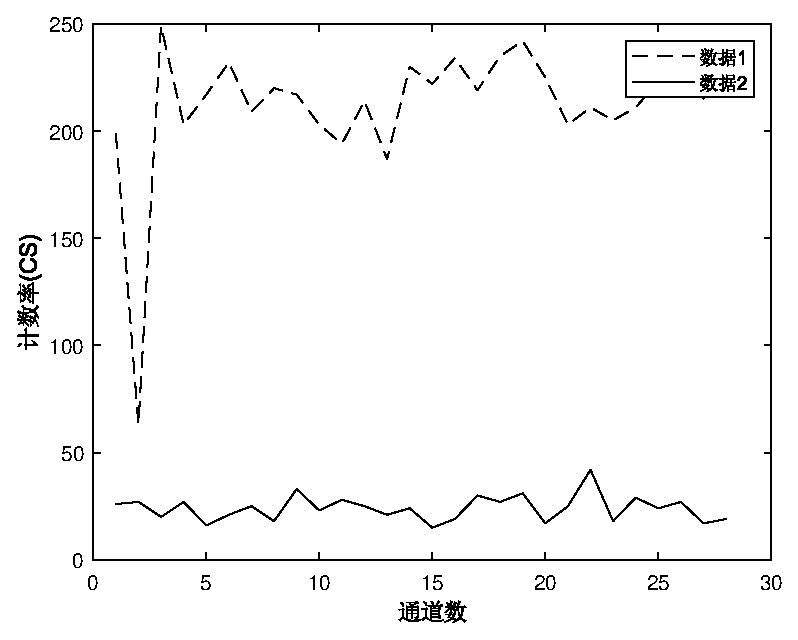
\includegraphics{channel.eps}
	\figcaption{通道与计数分布}\label{channel}
	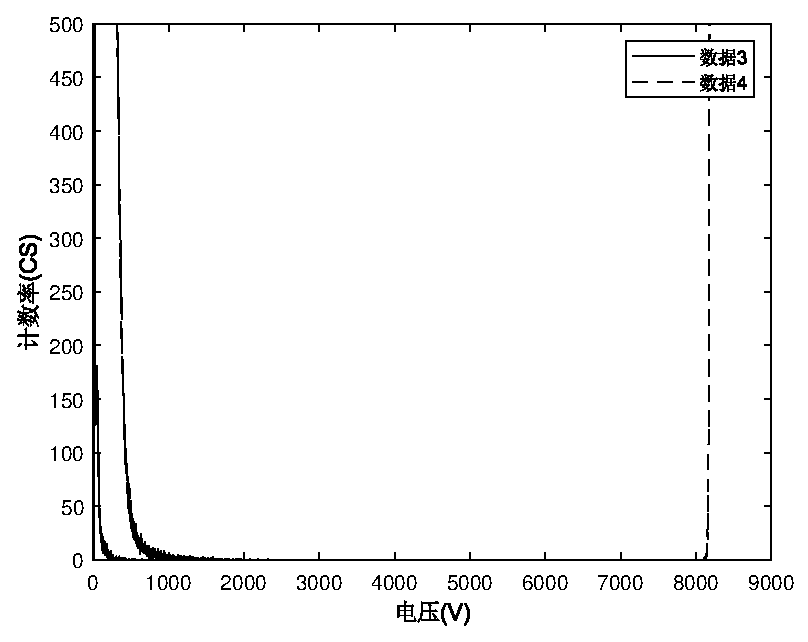
\includegraphics{voltage.eps}
	\figcaption{电压与计数分布}\label{voltage}
	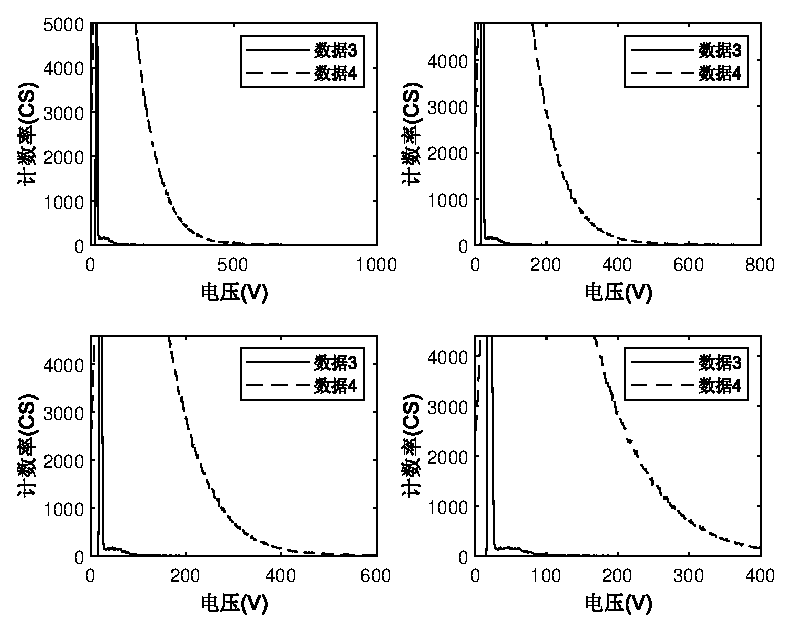
\includegraphics{voltagesub.eps}
	\figcaption{电压与计数分布(在更小范围内)}\label{voltagesub}
\end{center}
\section{实验结果分析}
 当被检测的光非常微弱时,光显示了粒子性。可以认为光电检测器接收的是单个离散的光子,相应的电信号就是离散的电脉冲信号,因而可以用脉冲计数的方法检测。在弱光探测中,一般都采用光电倍增管作为光子到电子的变换器。光功率愈大,脉冲的平均速率愈高。当光功率足够强时,这些脉冲就相互重叠,连成一片,而具有显著的直流分量。这是因为光电倍增管系量子探测器件,一个个光子撞击到光阴极上,产生光电发射,经倍增后,在阳极上便可释放出大量的电荷而形成脉冲。脉冲宽度与渡越时间分散及光电倍增管输出回路的时间常数有关。当后者与前者相比小得可以忽略时,则脉宽主要由渡越时间分散决定,一般为10-30毫微秒左右。此脉冲的平均速率与光子流的速率成一定的比例,故而我们只要在一定时间内计数此光电子脉冲,便等于检测了光流的强度。由此构成一种新的弱光检测方法,即光子计数。
 
 在图2中,最后的一部分上升的峰值是器件的阈值位置。
 \section{实验代码}
 	\lstinputlisting[language={MATLAB},
 numbers=left, numberstyle={\normalsize },	commentstyle=\color{red!50!green!50!blue!50}, 
 frame=shadowbox, rulesepcolor=\color{red!20!green!20!blue!20}]
 {code/Exp9.m}
\section{整体实验装置}
核心设备:
计数光电倍増管(包括管套和冷却器),高压电源(2000伏),脉冲前置放大器,甄别器,计数卡,光衰减器,普通光源,小孔,低压电源,脉冲幅度分析器,机箱等。

\section{实验内容及步骤}
\begin{enumerate}
	\item 用宽带存储示波器分别观察光电倍增管输出脉冲,分辦观察光电倍增管的直接输出(如果示波器灵度足够高的话)、放大器输出、甑别后的输出脉冲形状和高度。
	\item 辐照微弱光到光电倍增管上,重复上述步骤,检查光子脉冲与暗脉冲的差别。
	\item 在无光的情况下,调节甑别器到不同的阀值,给出该光电倍增管暗脉冲计数对幅度的分布
	\item 测量在有光情况下,光电倍增管的输出脉冲幅度分布曲线(需另备脉冲幅度分析器或多道分析器),找出其腰部位置,确定值甑别电平的高度,并与实际调节经验进行比较。
	\item 测量暗计数与光阴极温度间的关系。
	\item 选择一种光源输出波形,实测出光强变化曲线。
	\item 光子计数的其他应用实验(量子光学或时间分辨光谱一需要另外配各时幅转换器等)
\end{enumerate}

\end{document}